
\documentclass[twoside]{article}

\usepackage[square, numbers, comma, sort&compress]{natbib}
\usepackage{amsmath}
\usepackage{siunitx}
\usepackage{graphicx} % Required for the inclusion of images


\usepackage{lipsum} % Package to generate dummy text throughout this template

\usepackage[sc]{mathpazo} % Use the Palatino font
\usepackage[T1]{fontenc} % Use 8-bit encoding that has 256 glyphs
\linespread{1.05} % Line spacing - Palatino needs more space between lines
\usepackage{microtype} % Slightly tweak font spacing for aesthetics

\usepackage[hmarginratio=1:1,top=32mm,columnsep=20pt]{geometry} % Document margins
\usepackage{multicol} % Used for the two-column layout of the document
\usepackage[hang, small, labelfont=bf, up,textfont=it,up]{caption} % Custom captions under/above floats in tables or figures
\usepackage{booktabs} % Horizontal rules in tables
\usepackage{float} % Required for tables and figures in the multi-column environment - they need to be placed in specific locations with the [H] (e.g. \begin{table}[H])
\usepackage[hidelinks]{hyperref} % For hyperlinks in the PDF

\usepackage{lettrine} % The lettrine is the first enlarged letter at the beginning of the text
\usepackage{paralist} % Used for the compactitem environment which makes bullet points with less space between them

\usepackage{abstract} % Allows abstract customization
\renewcommand{\abstractnamefont}{\normalfont\bfseries} % Set the "Abstract" text to bold
\renewcommand{\abstracttextfont}{\normalfont\small\itshape} % Set the abstract itself to small italic text

\usepackage{titlesec} % Allows customization of titles
\renewcommand\thesection{\Roman{section}} % Roman numerals for the sections
\renewcommand\thesubsection{\Roman{subsection}} % Roman numerals for subsections
\titleformat{\section}[block]{\large\scshape\centering}{\thesection.}{1em}{} % Change the look of the section titles
\titleformat{\subsection}[block]{\large}{\thesubsection.}{1em}{} % Change the look of the section titles

\usepackage{fancyhdr} % Headers and footers
\pagestyle{fancy} % All pages have headers and footers
\fancyhead{} % Blank out the default header
\fancyfoot{} % Blank out the default footer
\fancyhead[C]{Variational Monte Carlo (VMC) for ICCP $\bullet$ April 2014 $\bullet$ AP3081D} % Custom header text
\fancyfoot[RO,LE]{\thepage} % Custom footer text

%----------------------------------------------------------------------------------------
%	TITLE SECTION
%----------------------------------------------------------------------------------------

\title{\vspace{-15mm}\fontsize{24pt}{10pt}\selectfont\textbf{Determining the ground-state energy of the hydrogen molecule with VMC}} % Article title

\author{
\large
\textsc{Bas \textsc{Nijholt}}\\[2mm] % Your name
\normalsize Delft University of Technology \\ % Your institution
\normalsize \href{mailto:bas@nijholt.biz}{bas@nijholt.biz} % Your email address
\vspace{-5mm}
}
\date{}

%----------------------------------------------------------------------------------------

\begin{document}

\maketitle % Insert title

\thispagestyle{fancy} % All pages have headers and footers

%----------------------------------------------------------------------------------------
%	ABSTRACT
%----------------------------------------------------------------------------------------

\begin{abstract}

\noindent The potential-energy curve for the electronic ground state of the hydrogen molecule has been calculated using the variational quantum Monte Carlo (QMC) method of solving the Schr\"odinger equation, with the use of the Born-Oppenheimer. The wavefunction sampling was carried out in a 6-dimensional configuration space of the four particles (two electrons and two protons.  % Dummy abstract text

\end{abstract}

%----------------------------------------------------------------------------------------
%	ARTICLE CONTENTS
%----------------------------------------------------------------------------------------

\begin{document}%{1} % Two-column layout throughout the main article text

\section{Introduction}
The determination of energies for molecular systems is a problem of general interest in chemistry and physics. We report here calculations of the ground state energy for the simplest molecular system containing a electron pair bond using the Variational Monte Carlo (VMC) method using the Born-Oppenheimer approximation. Accurate potential energy curves as functions of the inter-atomic distance have been computed for the ground state of the hydrogen molecule. \\

These calculations also provide us with an example of a computationally demanding problem which is well suited for parallel computing.\\ 

There is a long history of increasingly accurate theoretical calculations of the energy of the hydrogen molecule and increasingly accurate experimental measurements of the dissociation energy. The history of accurate calculations of energies for H$_2$ begins with the 1933 work of James and Coolidge \citep{james1933ground} which represented one of the first successes in solving the Schr\"odinger equation for molecules. In the 1960's, more accurate results for the hydrogen molecule were obtained by Kolos and Roothaan \citep{kolos1960accurate} and by Kolos and Wolniewicz \citep{kolos1963nonadiabatic, kol1964accurate, kol1965potential, kolos1968improved} which established the foundation for future calculations. \\

The effectiveness of the VMC method is demonstrated by applying it to a very simple quantum mechanical system, the harmonic oscillator from which we know the exact results.

\section{Variational Monte Carlo}
Variational Monte Carlo (VMC) is based on a direct application of Monte Carlo integration to explicitly correlated many-body wavefunctions. The variational principle of quantum mechanics, derived in the following section, states that the energy of a trial wavefunction will be greater than or equal to the energy of the exact wavefunction. Optimised forms for many-body wavefunctions enable the accurate determination of expectation values.

\subsection{Variational principle}
In quantum mechanics, the variational method is one way of finding approximations to the lowest energy eigenstate or ground state, and some excited states. The basis for this method is the variational principle \citep{griffiths1995introduction, sakurai1994modern}. The method consists in choosing a "trial wavefunction" depending on one or more parameters, and finding the values of these parameters for which the expectation value of the energy is the lowest possible. The wavefunction obtained by fixing the parameters to such values is then an approximation to the ground state wavefunction, and the expectation value of the energy in that state is an upper bound to the ground state energy.\\

The variational principle of quantum mechanics may be derived by expanding a normalized trial wavefunction, $\psi_{T}$, in terms of the exact normalized eigenstates of the Hamiltonian

\begin{equation}
 \psi_T=\sum_{i=0}^{\infty} c_{i} \psi_i \;\;\;,
\end{equation}

where the expansion coefficients, $c_{i}$, are normalised 

\begin{equation}
\sum_{i=0}^{\infty} \vert c_{i}\vert^2=1 \;\;\;.
\end{equation}

The expectation of the many-body Hamiltonian, $\hat{H}$, may be evaluated 

\begin{align}
 <\psi_T\vert\hat{H}\vert\psi_T >  = <\sum_i c_i\psi_i\vert\hat{H}\vert\sum_j c_j\psi_j > \\
 = \sum_i \sum_j c_{i}^{*} c_{j} \epsilon_{i} = \sum_i \vert c_{i}\vert^{2} \epsilon_{i}
\end{align}
where 
\begin{equation}
 \epsilon_{i} = <\psi_i\vert\hat{H}\vert\psi_i >
\end{equation}

The expectation value of a trial wavefunction with the Hamiltonian must therefore be greater than or equal to the true ground state energy.

\subsection{Monte Carlo integration}
Before the expectation value of a trial wavefunction with the many-body Hamiltonian may be computed, the integral must be transformed into a form suitable for Monte Carlo integration. Trial wavefunctions, $\psi_T$, are dependent on the set of $N$ electron positions,  ${\bf R}=\{{\bf r}_1,{\bf r}_2, \ldots {\bf r}_N\}$. The expectation value is given by

\begin{equation}
E=\frac{\int \psi_{T}^{*}\hat{H}\psi_{T} d{\bf R}}
{\int \psi_{T}^{*}\psi_{T}d{\bf R}}
\end{equation}

which may be rewritten in an importance sampled form in terms of the probability density  $\vert\psi_{T}\vert^{2}$ as

\begin{equation}
E=\frac{\int \vert\psi_{T}\vert^{2}\frac{\hat{H}\psi_{T}}{\psi_{T}} d{\bf R}}
{\int \vert\psi_{T}\vert^{2}d{\bf R}}
\end{equation}

The Metropolis algorithm samples configurations - sets of electron positions ${\bf R}$ - from the probability distribution  $\vert\psi_{T}\vert^{2}$, and the variational energy is obtained by averaging the ''local energy'' $E_{L}$ over the set of configurations $\{{\bf R}\}$ as 

\begin{equation}
\label{E_local}
E_{L}({\bf R})=\frac{\hat{H}\psi_{T}({\bf R})}{\psi_{T}({\bf R})}
\end{equation}

and 

\begin{equation}
E=\frac{1}{N} \sum E_{L}({\bf R}_i) \;\;\;.
\end{equation}

\subsection{Calculation procedure}
The program is written in Fortran 90 and implements VMC to solve the  problem of the hydrogen molecule using the trial wavefunction specified by equation (\ref{wf}). The program calculates the electronic eigenvalue (energy of the electrons). As soon as the compilation and the execution are successful, equation (\ref{cusp}) is solved for $a$ and the initial configuration is generated. The program commences by thermalising the walkers generated by the metropolis algorithm. The program will loop trough different values of $s$ and minimizes the energy for each distance by using a simple damped steepest decent method \citep{thijssen2007computational}

\begin{equation}
 \beta_{new}=\beta_{old}-\gamma \left( \frac{dE}{d\beta} \right)
\end{equation}

with 

\begin{equation}
\frac{dE}{d\beta}= 2\left(  \left\langle E_L \frac{d \ln \psi_T }{d \beta} \right\rangle - \left\langle \frac{d \ln \psi_T}{d \beta} \right\rangle \right)
\end{equation}
The calculations for different $s$ values are independent of each other, this makes this problem perfectly suited for parallel programming. The implementation led to speed-ups that scaled linear with the number of available cores.

The VMC algorithm consists of two distinct phases. In the first a walker consisting of an initially random set of electron positions is propagated according to the Metropolis algorithm, in order to equilibrate it and begin sampling $\vert\Psi\vert^2$. In the second phase, the walker continues to be moved, but energies and other observables are also accumulated for later averaging and statistical analysis. The procedure is as follows \citep{thijssen2007computational}.

  \begin{enumerate}
    \item Generate initial configuration using random positions for the electrons
    \item For every electron in the configuration:
    \begin{enumerate}
     \item Propose a move from ${\bf r}$ to  ${\bf r}^\prime=\bf r +\Delta$ 
     \item Compute  $w=\vert\Psi({\bf r}^\prime)/\Psi({\bf r})\vert^2$
     \item Accept or reject move according to Metropolis probability $\mathrm{min}(1,w)$
     \item After equilibration phase accumulate the contribution to the local energy according to equation (\ref{E_local})
    \end{enumerate}
    \item Repeat step 2 until sufficient data accumulated 
  \end{enumerate}

The Metropolis step size $\Delta$. must be chosen carefully. If it is too small, then random walkers will not visit regions far from their starting point, which will produce an insufficient sampling. On the other hand, too large a step size will bring about a low acceptance probability of particle movement, which will yield an inefficient sampling. Therefore, to make the Monte Carlo sampling both sufficient and efficient, it is reasonable to set the value of the step size so that the acceptance probability is fixed to be about 50\% throughout the simulation.

The evaluation of the local energy is done at every step after the equilibration phase in the course of the random walk of particles. The energies are data-blocked over an interval that is long enough to eliminate the correlation between two local energies which are evaluated successively.

%The whole random walk is partitioned into $N$ blocks, each of which is sufficiently large in order that the average of $N_s$ samples in the block can be regarded as independent of the others.

\subsection{The local energy}

The local energy,  $E_{L}({\bf R})$, equation (\ref{E_local}) is one of the central quantities in quantum Monte Carlo (QMC) methods. It occurs in both the variational and diffusion Monte Carlo algorithms and its properties are exploited to optimise trial wavefunctions. The local energy has the useful property that for an exact eigenstate of the Hamiltonian, the local energy is constant. For a general trial wavefunction the local energy is not constant and the variance of the local energy is a measure of how well the trial wavefunction approximates an eigenstate \citep{phd}. \\

Determination of the local energy is one of the most computationally costly operations performed in QMC calculations. Application of the Hamiltonian to the trial wavefunction requires computation of the second derivatives of the wavefunction and the calculation of the electron-electron and electron-ion potentials.

\subsection{Trail wavefunction}

The choice of trial wavefunction is critical in VMC calculations. All observables are evaluated with respect to the probability distribution  $\vert\Psi_T({\bf R})\vert^2$. The trial wavefunction,  $\Psi_T({\bf R})$, must well approximate an exact eigenstate for all ${\bf R}$ in order that accurate results are obtained. \\

Quantum Monte Carlo methods are able to exploit trial wavefunctions of arbitrary forms. Any wavefunction that is physical and for which the value, gradient and Laplacian of the wavefunction may be efficiently computed can be used\citep{phd}. \\

The power of Quantum Monte Carlo methods lies in the flexibility of the form of the trial wavefunction. In early studies the wavefunction was taken to be a Jastrow function \citep{jastrow1955many} which is of the form

\begin{equation}
\psi=\exp \left[ \sum_{i<j}^{N} -u(r_{ij}) \right] \;\;\;.
\end{equation}

\subsection{Hydrogen molecule \texorpdfstring{(H$_2$)}{Lg}}

The Hamiltonian of the Hydrogen molecule, in the Born-Oppenheimer approximation where we assume that the nuclear motion is negligible, includes the kinetic and potential energies of the two electrons as well as their interaction. The positions of the two atomic nuclei are assumed to be symmetrically located and on the x-axis at positions $-s/2$, $s/2$. The nuclei are thus $a$ distances apart. The positions of the two electrons are $\vec{r}_1$ and $\vec{r}_2$. The Hamiltonian (in convenient units) is then

\begin{align}
\label{Hamiltonian}
 \hat{H}=-\frac{1}{2}\left( \nabla_1^2 + \nabla_2^2 \right) +\frac{1}{\left| \vec{r}_{12} \right|}  \\ - \left[ \frac{1}{|\vec{r}_{1L}|} +\frac{1}{|\vec{r}_{1R}|}+\frac{1}{|\vec{r}_{2L}|}+\frac{1}{|\vec{r}_{2R}|} \right] 
\end{align}

where the first part is the kinetic energy of the two electrons, the second part is the Coulomb repulsion between the two electrons and the last term (square brackets) is the four attraction terms between the two electrons and the two nuclei. And in which $\vec{r}_{1L} = \vec{r}_1 + \frac{s}{2} \hat{i}$, $\vec{r}_{1R} = \vec{r}_1 - \frac{s}{2} \hat{i}$, $\vec{r}_{2L} = \vec{r}_2 + \frac{s}{2} \hat{i}$, $\vec{r}_{1R} = \vec{r}_2 - \frac{s}{2} \hat{i}$ and $\vec{r}_{12} = \vec{r}_1 -\vec{r}_2$. The unit of length is in units of the Bohr radius $a_0=\frac{\hbar^2}{m_e k e^2}=\SI{0.529}{\angstrom}$ and the unit of energy is twice the ionization energy of the hydrogen atom $E=\frac{(ke^2)^2}{a_0}=\SI{27.2}{\electronvolt}$. The trail variational wavefunction is chosen to be 
\begin{equation}
\label{wf}
 \Psi_{T}(\vec{r}_1,\vec{r}_2)=\phi(\vec{r}_1)\phi(\vec{r}_2)\psi(\vec{r}_1,\vec{r}_2)
\end{equation}
where the interaction term $\psi(\vec{r}_1,\vec{r}_2)$ takes the form of the Jastrow function

\begin{equation}
\psi(\vec{r}_1,\vec{r}_2) = \psi_{12} = e^{\frac{\left| \vec{r}_{12}  \right|}{\alpha(1+\beta |\vec{r}_{12}|)} }
\end{equation}

with $\alpha$ and $\beta$ as variational parameters, and $\phi(\vec{r}_1) \equiv \phi_1$ and $\phi(\vec{r}_2) \equiv \phi_2$ are

\begin{equation}
 \phi_1 = e^{-|\vec{r}_{1L}|/a} + e^{-|\vec{r}_{1R}|/a} = \phi_{1L} +\phi_{1R}
\end{equation}

\begin{equation}
 \phi_2 = e^{-|\vec{r}_{2L}|/a} + e^{-|\vec{r}_{2R}|/a} = \phi_{2L} +\phi_{2R}
\end{equation}

At this point there are four parameters in the variational problem $s$, $a$, $\alpha$, $\beta$. We can remove one of two of them by using the so-called Coulomb cusp conditions. These are required to ensure that there is no singularity in the energy when either electron approaches either proton, or when the two electrons are at the same position. The four cases of an electron approaching a proton lead to the same condition 
\begin{equation}
\label{cusp}
 a(1+e^{-s/a}) =1
\end{equation}
while the case of two electrons approaching each other lead to the condition $\alpha=2$. The local energy is \footnote{for the full derivation of the local energy, the Coulomb cusp condition and the Hamiltonian see the appendix}

 \begin{multline}
 E_L =  \frac{1}{a\phi_1}\left[ \frac{\phi_{1L}}{r_{1L}}+\frac{\phi_{1R}}{r_{1R}} \right] + \frac{1}{a\phi_2} \left[ \frac{\phi_{2L}}{r_{2L}}+\frac{\phi_{2R}}{r_{2R}}\right] \\
 + \left(  \frac{\phi_{1L}\hat{r}_{1L}+\phi_{1R}\hat{r}_{1R}}{\phi_1}   -    \frac{\phi_{2L}\hat{r}_{2L}+\phi_{2R}\hat{r}_{2R}}{\phi_2}     \right)  \cdot \\ 
 \frac{\hat{r}_{12}}{2 a(\beta r_{12}+1)^2} +\frac{1}{\left| \vec{r}_{12} \right|}  \\
  -   \frac{(1+4 \beta) r_{12} + 4}{4r_{12}(\beta r_{12}+1)^4}  - \frac{1}{a^2} \\
  - \left[ \frac{1}{|\vec{r}_{1L}|} +\frac{1}{|\vec{r}_{1R}|}+\frac{1}{|\vec{r}_{2L}|}+\frac{1}{|\vec{r}_{2R}|} \right] 
\end{multline}

%------------------------------------------------

\section{Results}
To test the capabilities of our analytical ansatz to correctly describe the hydrogen molecule we first consider the ground-state energy for the quantum harmonic oscillator whose exact wavefunction as well as eigenvalue is known.

\begin{table}[H]
\caption{Variational Monte Carlo energies}
\label{table:HO}
\centering
\begin{tabular}{lllll}
$\alpha$ & $\left\langle E \right\rangle$ & $\operatorname{Var}(\left\langle E \right\rangle)$ & $E_v$ & $\operatorname{Var}(E)_v$ \\
\midrule
$0.4$  & $0.5124$ & $0.0255$  & $0.5125$  & $0.0253$ \\
$0.45$ & $0.5027$ & $0.00556$ & $0.50278$ & $0.0056$\\
$1/2$  & $1/2$    & 0         & $1/2$     & 0 \\
$0.55$ & $0.5022$ & $0.0045$  & $0.5022$  & $0.0045$\\
$0.6$  & $0.5084$ & $0.0166$  & $0.5083$  & $0.0168$
\end{tabular}
\caption*{VMC energies are given for the harmonic oscillator for various values of the variational parameters. 1000 walkers have been used and 100 000 displacements were attempted. The first 10 000 were removed from the data to ensure equilibrium. The expectation value for the energy $\left\langle E \right\rangle$ and the variance $\operatorname{Var}(\left\langle E \right\rangle)$ are given, the analytical values $E_v$ and $\operatorname{Var}(E)_v$ are also given.}
\end{table}

The results are summarized in table \ref{table:HO}. For details on the simulation we refer the reader to the appendix. \\

\begin{figure}[H]
 \centering
 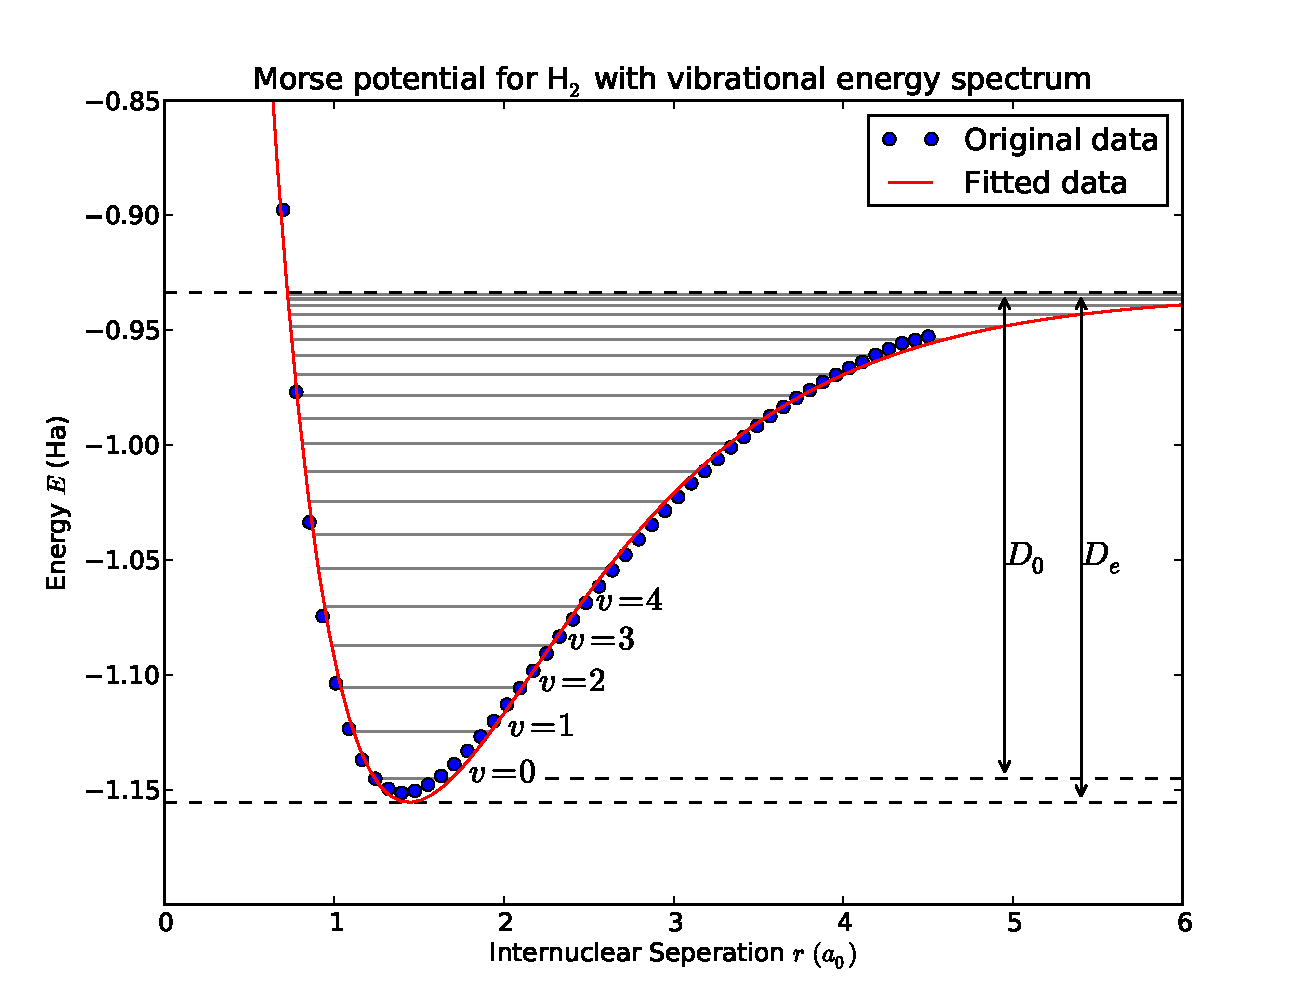
\includegraphics[width=\linewidth]{plot.pdf}
 \captionof{figure}{The Morse potential (solid red) fitted to the data (blue dots). The fitting parameters are $r_e=1.441(6)$, the equilibrium bond distance with a corresponding energy of $E_0=-1.155(1)$, $D_e=0.221(2)$ the well depth and $a=0.97(1)$ the width of the well.}\label{fig:plot}
\end{figure}

Our goal was to solve the six-dimensional partial differential eigenvalue equation for the lowest eigenvalue $E_0$ at different inter-proton separation distances $s$, and so trace out the potential $V(s)$. This potential should look much like the Morse potential; the depth and location of the minimum and the curvature of $V$ about this minimum are related to observable properties of the H$_2$ spectrum. The ground-state energy was calculated for 50 different values of $s$, after which the Morse potential, $V(r) = D_e ( 1-e^{-a(r-r_e)} )^2$, was fitted to the data. The results are depicted in figure \ref{fig:plot} and summarized in table \ref{H2}. In order to find the dissociation energy of H$_2$, we look at $D_e$, the depth of the well in the Morse potential and subtract the energy of two isolated hydrogen atoms in its ground-state. In table \ref{D_e} our value is compared to experimental values and to values found with different methods. Units of cm$^{-1}$ are used as it is an industry standard.

\begin{table}[H]
\caption{Results of H$_2$}
\label{H2}
\centering
\begin{tabular}{llr}
\hline
Reference   &  & Energy      \\ \hline
Exp.        & Herzberg \citep{herzberg1970dissociation}   & $36 117.3 \pm 1.0$ \\
Exp.        & Stwalley \citep{stwalley1970dissociation}   & $36 118.6 \pm 0.5$  \\
Nonadiabatic& Wolniewicz \citep{wolniewicz1983x}          & $36 118.1 \pm 0.5$ \\
Nonadiabatic& Kolos \citep{szalewicz1986new}              & $36 118.01 \pm 0.5$ \\
DQMC        & Traynor \citep{traynor1991quantum}          & $36 107 \pm 11$ \\
GFQMC       & Traynor \citep{traynor1991quantum}          & $36 118.6 \pm 2.0$ \\
VMC         & This work                                   & $36 219.8 \pm 70$  \\ \hline
\end{tabular}
\end{table}

\begin{table}[H]
\caption{Comparing the dissociation energy of H$_2$ ($D_0$)}\label{D_e}
\centering
\begin{tabular}{llr}
\hline
Reference   &  & Energy      \\ \hline
Exp.        & Herzberg \citep{herzberg1970dissociation}   & $36 117.3 \pm 1.0$ \\
Exp.        & Stwalley \citep{stwalley1970dissociation}   & $36 118.6 \pm 0.5$  \\
Nonadiabatic& Wolniewicz \citep{wolniewicz1983x}          & $36 118.1 \pm 0.5$ \\
Nonadiabatic& Kolos \citep{szalewicz1986new}              & $36 118.01 \pm 0.5$ \\
DQMC        & Traynor \citep{traynor1991quantum}          & $36 107 \pm 11$ \\
GFQMC       & Traynor \citep{traynor1991quantum}          & $36 118.6 \pm 2.0$ \\
VMC         & This work                                   & $36 219.8 \pm 70$  \\ \hline
\end{tabular}
\end{table}

asda




%------------------------------------------------

\section{Discussion}
The present approach has provided good results for the small systems treated here. Especially, the error is within about 0.2\% of the exact energy when one utilizes a trial wavefunction for which 0.998, and such a trial wavefunction can generally be obtained by multiplying a Hartree-Fock single. determinant of a single-zeta basis by a simple electron-electron Jastrow factor. So, it seems useful to apply the CMX-VMC method to the calculation of electronic energies and other physical quantities of larger systems.

\subsection{Subsection Two}


%----------------------------------------------------------------------------------------
%	REFERENCE LIST
%----------------------------------------------------------------------------------------

% \begin{thebibliography}{99} % Bibliography - this is intentionally simple in this template
% 
% \bibitem[Figueredo and Wolf, 2009]{Figueredo:2009dg}
% Figueredo, A.~J. and Wolf, P. S.~A. (2009).
% \newblock Assortative pairing and life history strategy - a cross-cultural
%   study.
% \newblock {\em Human Nature}, 20:317--330.
%  
% \end{thebibliography}

\bibliography{mybib}{}
\bibliographystyle{plain}


%----------------------------------------------------------------------------------------

\end{multicols}

\end{document}
